\documentclass[a4paper, 10pt, french]{article}
% Préambule; packages qui peuvent être utiles
   \RequirePackage[T1]{fontenc}        % Ce package pourrit les pdf...
   \RequirePackage{babel,indentfirst}  % Pour les césures correctes,
                                       % et pour indenter au début de chaque paragraphe
   \RequirePackage[utf8]{inputenc}   % Pour pouvoir utiliser directement les accents
                                     % et autres caractères français
   \RequirePackage{lmodern,tgpagella} % Police de caractères
   \textwidth 17cm \textheight 25cm \oddsidemargin -0.24cm % Définition taille de la page
   \evensidemargin -1.24cm \topskip 0cm \headheight -1.5cm % Définition des marges
   \RequirePackage{latexsym}                  % Symboles
   \RequirePackage{amsmath}                   % Symboles mathématiques
   \RequirePackage{tikz}   % Pour faire des schémas
   \RequirePackage{graphicx} % Pour inclure des images
   \RequirePackage{listings} % pour mettre des listings
% Fin Préambule; package qui peuvent être utiles

\title{Rapport de TP 4MMAOD : Génération de patch optimal}
\author{
{\sc Gouttefarde} Léo (groupe 5)\\
{\sc Piellard} Jérémie (groupe 2)
}
\begin{document}

\maketitle

%%%%%%%%%%%%%%%%%%%%%%%%%%%%%%%%%%%%%%%%%%%%%%
\section{Principe de notre  programme}
Nous avons choisi le C\texttt{++} car nous voulions obtenir de bonnes performances
et que nous avons jugé un langage orienté objet bien adapté au problème.\\

Nous avons écrit la classe \texttt{File} pour accéder aux fichiers d'entrée et de sortie. Pour limiter les défauts de cache et éviter des accès au disque moins fréquents, nous les chargeons entièrement en mémoire.\\

Pour le calcul du patch optimal, nous avons créé la classe \texttt{Solver}.
Cette classe résout l'équation de Bellman de manière itérative.

On crée un tableau d'états de taille $(n_1+1)\times(n_2+1)$.
Un état est représenté par la donnée d'un coût optimal et de l'opération nécessaire pour arriver dans cet état
(on peut en déduire l'état précédent), soit deux entiers.

On commence par remplir les conditions aux bords :
\begin{itemize}
\item état $(0,j)$ accessible uniquement par $j$ additions;
\item état $(i,0)$ accessible uniquement par destructions.
\end{itemize}

Ensuite on calcule les autres coûts en parcourant la matrice par ligne
(c'est-à-dire à $j$ constant).
Le calcul du coût de l'addition, la substitution ou la destruction sont simples.
Pour le coût de la multi-destruction, on retient l'indice le plus avantageux
et on le met à jour à chaque incrémentation de $i$ (cela évite de parcourir une nouvelle fois toute la ligne).\\

Quand la matrice des états est remplie, pour écrire le patch optimal on part de l'état $(i_{max}, j_{max})$
et on remonte la suite des instructions effectuées pour retrouver l'état $(0,0)$.
On stocke ces opérations dans une liste, que l'on parcourt à nouveau afin d'écrire le patch final.

%%%%%%%%%%%%%%%%%%%%%%%%%%%%%%%%%%%%%%%%%%%%%%
\section{Analyse du coût théorique}

  \subsection{Nombre  d'opérations en pire cas\,: }
    Il est en $\Theta(n_1 n_2)$.\\

    \textbf{Justification\,:} Pour calculer les coûts, on parcourt exactement une fois le tableau the taille $((n_1 +1)\times(n_2 +1))$.
    Le traitement de chaque case a un coût fixe car on teste systématiquement les 4 opérations possibles (sauf pour les cases $i=0$ ou $j=0$ qui ont un coût moindre).

    Le coût de lecture des fichiers d'entrée et de sortie ($\Theta(n_1)$ et $\Theta(n_2)$ respectivement) sont négligeables.

    Enfin le coût d'écriture du patch est en pire cas en $\Theta(n_2)$ puisque le patch est au plus constitué de $2n_2$ lignes.

  \subsection{Place mémoire requise\,: }
    Il est en $\Theta(n_1 n_2)$.\\

    \textbf{Justification\,:} On stocke entièrement les deux fichiers en mémoire : coût $\Theta(c_1 + c_2) = o(n_1n_2)$.

    On a également besoin de stocker un tableau $(n_1+1)\times(n_2+1)$ : coût $\Theta(n_1n_2)$.

    Enfin pour l'écriture du patch on utilise temporairement une liste de taille maximale $n_1 + n_2$ : coût $\Theta(n_1 + n_2) = o(n_1n_2)$.

  \subsection{Nombre de défauts de cache sur le modèle CO\,: }
  	Le nombre de défauts de cache est en $\Theta \left (\frac{n_1n_2}{L} \right )$, où $L$ est la longueur d'une ligne de cache et en supposant $2 \, n_1 < L$.\\
  	
     \textbf{Justification\,:} On parcourt itérativement un tableau de taille $n_1n_2$. Cependant on accède à deux lignes adjacentes en même temps (pour tester l'addition notamment). En supposant $2 \, n_1 < L$, cela n'a pas d'influence sur les défauts de cache.


%%%%%%%%%%%%%%%%%%%%%%%%%%%%%%%%%%%%%%%%%%%%%%
\section{Compte rendu d'expérimentation}
  \subsection{Conditions expérimentales}

    \subsubsection{Description synthétique de la machine\,:} 

    La machine utilisée pour notre test est une machine de la salle E203.
    Cette machine a un processeur Intel Core i5 4 coeurs à 3,3 Ghz et 16 Go de mémoire RAM.

    \subsubsection{Méthode utilisée pour les mesures de temps\,: } 

    Le code a été compilé avec l'option -O3.
    Les mesures sont effectuées dans le code C++ lui-même (et pas dans le Makefile).
    Pour que ces mesures prennent en compte la désallocation mémoire, nous avons
    alloué et désalloué manuellement une instance de notre solveur.

    Nous avons fait alterné les tests pour faire les mesures pour éviter que
    le système d'exploitation mette en cache les fichiers ce qui aurait faussé les temps d'exécution.
    Cependant nous obtenons des mesures semblables en passant 5 fois le même test à la suite.

    Les mesures sont en millisecondes.
    Il faut noter que la machine offre une précision de mesure maximale de 20 ms.

  \subsection{Mesures expérimentales}

    \begin{figure}[h!]
      \begin{center}
        \begin{tabular}{|l||r||r|r|r||}
          \hline
          \hline
            & coût         & temps     & temps   & temps \\
            & du patch     & min       & max     & moyen \\
          \hline
          \hline
            benchmark 1 & 2540 & 20 & 20 & 20 \\
          \hline
            benchmark 2 & 3120 & 80 & 90 & 82 \\
          \hline
            benchmark 3 & 809 & 160 & 180 & 170 \\
          \hline
            benchmark 4 & 1708 & 350 & 370 & 360 \\
          \hline
            benchmark 5 & 7553 & 460 & 470 & 468 \\
          \hline
            benchmark 6 & 37027 & 2050 & 2070 & 2060 \\
          \hline
          \hline
        \end{tabular}
        \caption{Mesures des temps minimum, maximum et moyen de 5 exécutions pour les 6 benchmarks.}
        \label{table-temps}
      \end{center}
    \end{figure}

\newpage
\subsection{Analyse des résultats expérimentaux}

Voici ci-dessous le graphe du temps d'exécution divisé par $NM$ en fonction de $NM$.
Nous avons créé nous même quelques patchs pour tester d'autres valeurs de $NM$ et compléter le graphe.
On constate que le temps d'exécution est bien proportionnel à la quantité $NM$.


\begin{figure}[h!]
\begin{center}
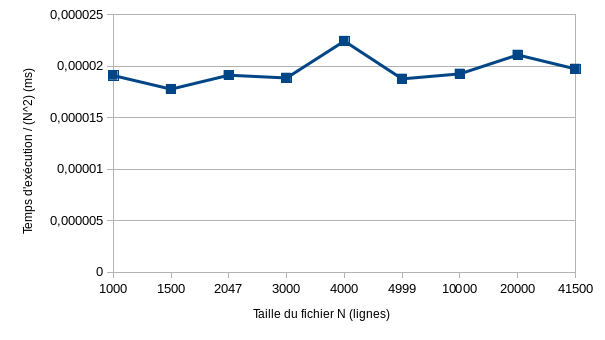
\includegraphics[width=12cm]{exec.png}
\caption{Temps d'exécution divisé par $NM$ en fonction de $NM$}
\end{center}
\end{figure}

%%%%%%%%%%%%%%%%%%%%%%%%%%%%%%%%%%%%%%%%%%%%%%
\section{Question\,: et  si le coût d'un patch était sa taille en octets ?}
    Dans le cas où le coût d'un patch est sa taille en octet,
on peut garder le même programme en changeant simplement le coût des opérations.
Les coûts deviennent:

\begin{itemize}
\item addition de la ligne j après la ligne k : $taille("+\ k\backslash n") + taille(ligne_j)$
\item substitution de la ligne j par la ligne k : $taille("=\ k\backslash n") + taille(ligne_j)$
\item suppression de la ligne i : $taille("d\ i\backslash n")$
\item suppression de n lignes après la ligne i : $taille("D\ i\ j\backslash n")$
\end{itemize}

% {\em Préciser le principe de la résolution choisie (parmi celles vues en cours); donner  les modifications à apporter (soit à vos  équations, soit à votre programme, au choix) 
% pour s'adapter à cette nouvelle fonction de coût. 
% }

\end{document}
%% Fin mise au format

